% file: kap_optocoupler.tex
%============================= Kapitola: Optoelektronika =====================================================
\chapter{Optoelektronika}\label{ES:kap_optocoupler}
\minitoc
\newpage
  \section{Optoelektronické systémy}
    Velmi rozšířené je využití fotonové vazby pro galvanické oddělení pomocí optoelektronických vazebních 
    členů, optronů, a přenos dat pomocí optických kabelů. Optron je tvořen zdrojem (obvykle GaAs LED) a 
    detektorem záření (obvykle Si fotodioda nebo Si fototranzistor) vzájemně spojených optickou vazbou v 
    jednom pouzdře. Vstup a výstup jsou proto elektricky odizolovány a podle typu pouzdra snesou izolační 
    napětí\footnote{(izolačním napětím se myslí rozdíl efektivních hodnot napětí mezi libovolnou vstupní a 
    výstupní svorkou, při kterém dochází k průrazu mezi vstupem a výstupem)} 1,5 kV až 5 kV.     
    \begin{figure}[ht!]  
      \centering
      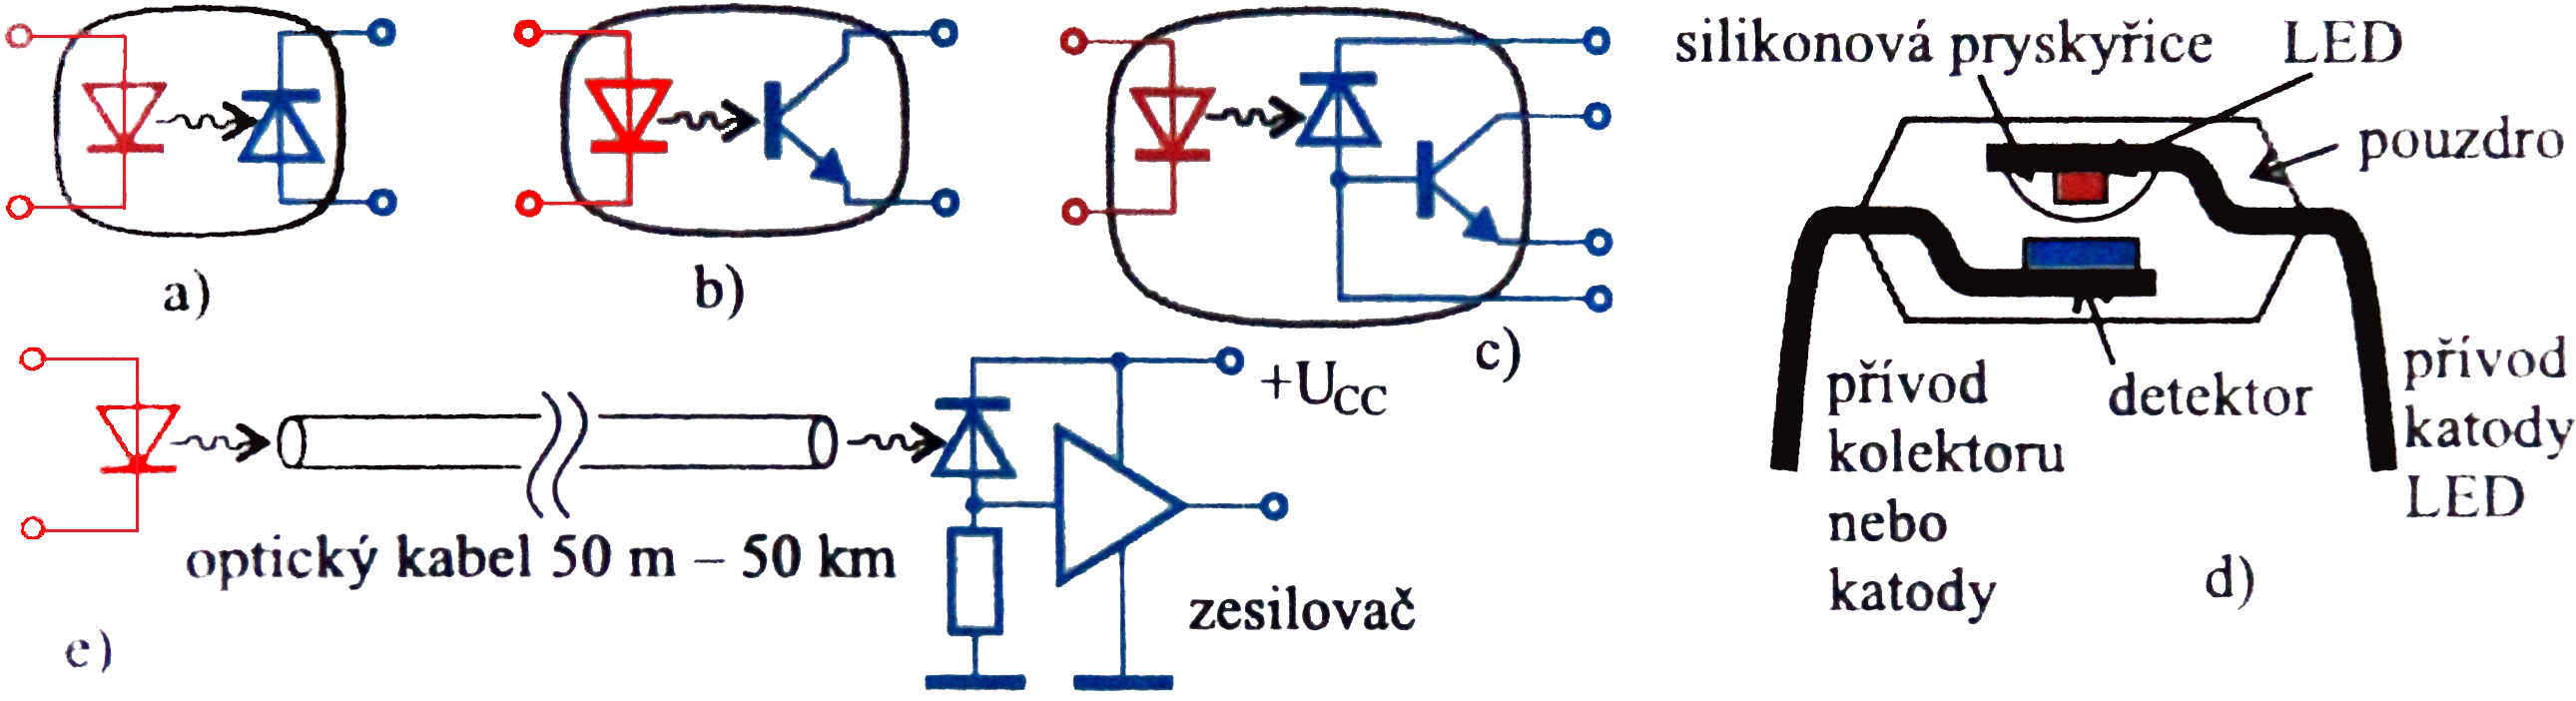
\includegraphics[width=\linewidth]{zahlava_optoel_sys.jpg}
      \caption{Optoelektronické systémy \cite[p.~179]{Zahlava2001}}
      \label{ES:fig_opto_sys}
    \end{figure}
  
    Přenos signálu mezi zdrojem a detektorem na velkou vzdálenost se provádí prostředím s malým útlumem a 
    vysokou šumovou imunitou, kterým je optické vlákno. Jedno nebo několik takových vláken s povrchovou a 
    mechanickou ochranou (z kevlaru a polyuretanu) tvoří optický kabel. Vlákno se skládá z vnitřního 
    skleněného jádra (o průměru jednotek až desítek \(\mu m\)) s indexem lomu \(n\), a je pokryto tenkým 
    skleněným pláštěm (tlustým desítky \(\mu m\)) s indexem lomu \(n_2\). Jelikož \(n_1>n2\), dochází pro 
    určité rozmezí úhlu dopadu k odrazu záření na rozhraní jádro-plášť a energie záření se pak šíří převážně 
    jádrem vlákna. Z důvodu nízkého útlumu vlákna se přenos uskutečňuje v přenosových oknech 
    \SI{850}{\nano\meter}, \SI{1300}{\nano\meter} a \SI{1550}{\nano\meter}, přičemž s rostoucí hodnotou 
    vlnové délky útlum vlákna klesá, ale cena potřebných optoprvků roste.
    
    \emph{Typy optronů z hlediska aplikace:}
      \begin{itemize}
        \item optrony vyráběné pro aplikace v lineárních obvodech mají dobrou linearitu a jsou
              používány pro galvanické oddělení analogových obvodů;
        \item optrony vyráběné pro aplikace v logických obvodech jsou určeny pro přenos pouze dvou
              úrovní signálů a proto je jejich realizace podstatně snadnější než realizace
              lineárních optronů.
      \end{itemize}
  
    \subsection{Statické parametry optoelektronických vazebních systémů}
      \subsubsection{Proudový přenosový poměr CTR}\label{ES:Opto_CTR}
        Přenosovou účinnost optoelektronického vazebního systému charakterizuje \emph{proudový
        přenosový poměr CTR} (Current Transfer Ratio), který udává poměr výstupního ku vstupnímu
        proudu optronu v procentech při daném pracovním napětí (nastavení pracovního bodu), zátěži a
        teplotě. 
        \begin{equation}\label{ES:eq_CTR1}
          CTR=\frac{I_{out}}{I_{in}}\times100  \qquad\text{[\%]} 
        \end{equation}
        S fotodiodou na výstupu je \(\text{CTR}\approx0,2-0,3\,\%\) a s fototranzistorem na výstupu
        je \(\text{CTR}\approx10-100\,\%\). Tento poměr vyjádřený rovnicí \ref{ES:eq_CTR1} je
        parametr svými vlastnostmi podobný proudovému zesilovacímu činiteli bipolárního tranzistoru
        \(h_{FE}\)\footnote{nebo též \(h_{21E}\) resp. \(\beta\). Jedná se o parametr vystupující
        v hybridních rovnicích popisující chování tranzistoru v zapojení se společným emitorem.
        \(h_{21E}\) jako diferenciální proudový přenos při výstupu nakrátko} a je s ním možné
        pracovat podobným způsobem.
               
        V následujích odstavcích se budeme předpokládat optoelektronický vazební systém s
        fotodiodou na vstupu a fototranzistorem na výstupu. V tomto případě je zřejmé, že CTR udává
        v procentech poměr velikosti kolektorového proudu přijímacího tranzistoru \(I_C\) ku proudu
        vysílací diodou \(I_F\).
        \begin{equation}\label{ES:eq_CTR2}
          CTR=\frac{I_{C}}{I_{F}}\times100  \qquad\text{[\%]} 
        \end{equation}
        Poměr je udáván pro určitý proud \(I_F\) diody LED a kolektorové napětí \(U_{CE}\)
        fototranzistoru, např. \(CTR = 50\,\%\) při \(I_F = \SI{1}{\milli\ampere}\), \(U_{CE} =
        \SI{5}{\volt}\) znamená, že když fotodiodou teče proud \(\SI{1}{\milli\ampere}\), je
        výstupní kolektorový proud \(I_F = \SI{0,5}{\milli\ampere}\).
        
        \begin{itemize}
          % CTR dependency on LED input current (IF)
          \item \emph{Závislost CTR na vstupním proudu fotodiody} na obr. \ref{ES:fig_opto_CTR01},
                není dáná monotónní funkcí, tj průběhem který by jen klesal, nebo naopak jen
                narůstal, ale vykazuje extrém, při kterém je dosažený přenosový poměr maximální.
                \begin{figure}[ht!]
                  \centering
                  \begin{tabular}{c}
                    \subfloat[Závislost CTR na vstupním proudu fotodiody]
                       {\label{ES:fig_opto_CTR01}
                        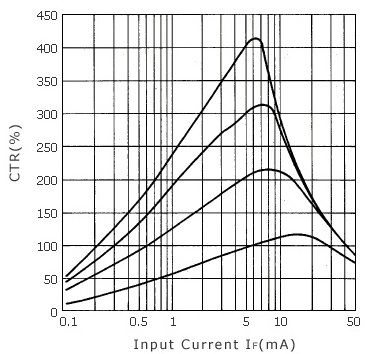
\includegraphics[width=0.8\linewidth]{ES_opto_CTR01.jpg} }   \\
                    \subfloat[Závislost CTR na teplotě]
                       {\label{ES:fig_opto_CTR03}
                        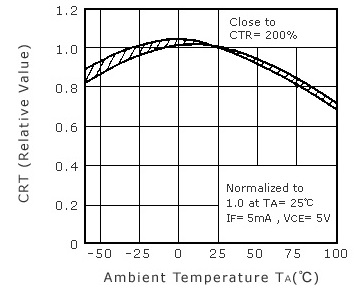
\includegraphics[width=0.8\linewidth]{ES_opto_CTR03.jpg} }
                  \end{tabular}    
                  \caption{Závislost CTR na vstupním proudu fotodiody a) a teplotě b)}
                  \label{ES:fig_opto_CTRparam}
                \end{figure}
          % CTR dependency on temperature      
          \item \emph{Závislost CTR na teplotě} na obr. \ref{ES:fig_opto_CTR02} ukazuje že
                zobrazená křivka je výsledkem kombinace dvou teplotních koeficintů. Zatímco
                světelná účinnost LED\footnote{LED luminous efficiency} vykazje záporný teplotní
                koeficient, tranzistor naproti tomu kladný teplotní koeficient.
                \ref{ES:fig_opto_CTR02}. 
                \begin{figure}[ht!]
                  \centering
                  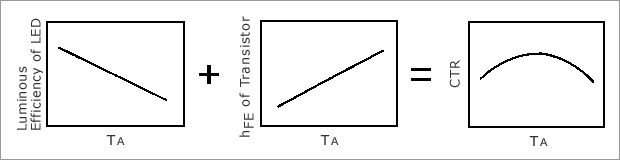
\includegraphics[width=\linewidth]{ES_opto_CTR02.jpg}
                  \caption{Závislost CTR na teplotě}
                  \label{ES:fig_opto_CTR02}
                \end{figure}
          % Change of CTR over operating time      
          \item \emph{Závislost CTR na čase} na obr. \ref{ES:fig_opto_CTR04} a obr.
                \ref{ES:fig_opto_CTR05} udává velice důležitou vlastnost, na kterou je třeba klást
                důraz v aplikacích, vyžadující dlouhou životnost produktu. Mohou to být
                například větrné elektrárny, drážní zabezpečovací zařízení atd. Největší vliv má na
                pokles CTR rychlost stárnutí fotodiody. Světelná účinnost klesá tím rychleji, čím
                větší je pracovní proud \(I_F\) viz obr. \ref{ES:fig_opto_CTR04} a čím větší je
                okolní teplota viz obr. \ref{ES:fig_opto_CTR05}. V určité formě je degradace CTR
                způsobena také stárnutím optické vazby mezi fotodiodou a fototranzistorem a změnou
                účinnosti foto-elektrické konverze a stejnosměrného zesílení
                samotného fototranzisotru tj. \(h_{FE}\).              
                % The change of the CTR over operating time is mainly caused by a drop in the
                % luminous efficiency of the LED. In general, the larger the LED input current (IF)
                % and the higher the ambient temperature, the faster the CTR decreases.
                \begin{figure}[ht!]
                  \centering
                  \begin{tabular}{c}
                    \subfloat[vliv pracovního proudu fotodiody \(I_F\)]
                      {\label{ES:fig_opto_CTR04}
                       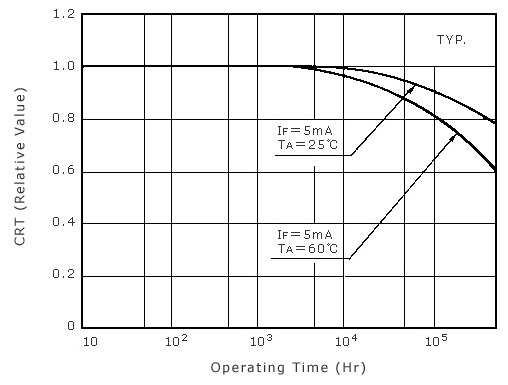
\includegraphics[width=0.8\linewidth]{ES_opto_CTR04.jpg}}   \\
                    \subfloat[Závislost CTR na provozní době]
                      {\label{ES:fig_opto_CTR05}
                       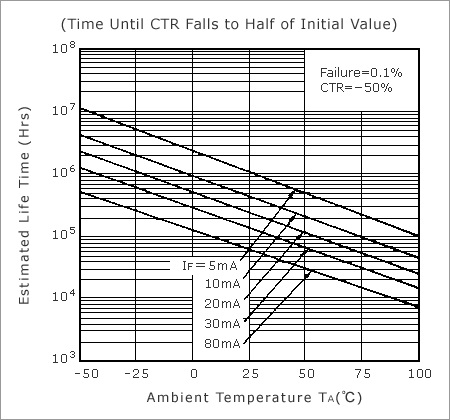
\includegraphics[width=0.8\linewidth]{ES_opto_CTR05.jpg}}   
                  \end{tabular}   
                  \caption{Závislost CTR na provozní době}
                  \label{ES:fig_opto_CTRtime}
                \end{figure}
        \end{itemize}      
      \       
      % -------------------Dynamické parametry optoelektronických vazebních systémů----------------  
      \subsection{Dynamické parametry optoelektronických vazebních systémů}
        Rychlost optronu je většinou limitována detektorem na výstupu. Pro rychlý přenos číslicového
        signálu se proto vyrábí optrony s fotodiodou integrovanou na jednom čipu s rychlým
        zesilovačem, jehož výstup je přímo slučitelný s číslicovými obvody. 
      %\subsection{Response time}       
        The response time of a photocoupler is similar to that of a transistor, and is expressed as
        follows. tf // RL X hFE X CCB kde \(R_L\ldots\) zatěžovací odpor, \(h_{FE}\ldots\) proudový
        zesilovací činitel tranzitoru (DC amplification) , \(C_{CB}\ldots\) kapacita mezi kolektorem
        a bází.
                      
        From this formula, tf increases as the load resistance increases as shown in Figure 6, so
        for high-speed signal transfer, the load resistance must be designed as small as possible
        within the allowable rating range.      
         \begin{figure}[ht!]
           \centering
           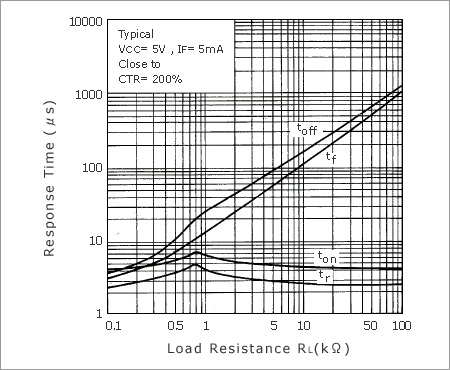
\includegraphics[width=0.9\linewidth]{ES_opto_CTR06.jpg}
           \caption{Response Time vs. RL Characteristics }
           \label{es:fig_opto_CTR06}
         \end{figure}      
      
         \begin{figure}[ht!]
           \centering
           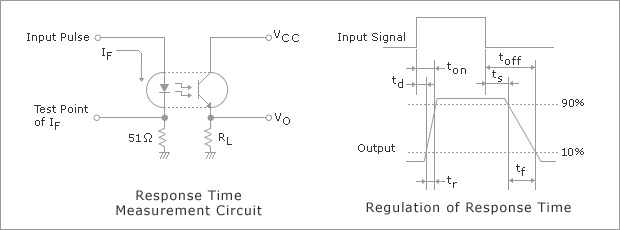
\includegraphics[width=0.9\linewidth]{ES_opto_CTR07.jpg}
           \caption{***}
           \label{es:fig_opto_CTR07}
         \end{figure}             
          However, when the load resistance is minimized, the transistor may not become completely
          ON and the output signal may be unstable unless the input current IF and output current IC
          are determined making sufficient allowance for factors such as the CTR specification
          range, the temperature characteristics, and the change over time.
                   
          Some examples of these characteristics are introduced below.      
                   
          Figure 7 shows an example of the variation in the response time according to the ambient
          temperature (TA).
         
          \begin{figure}[ht!]
            \centering
            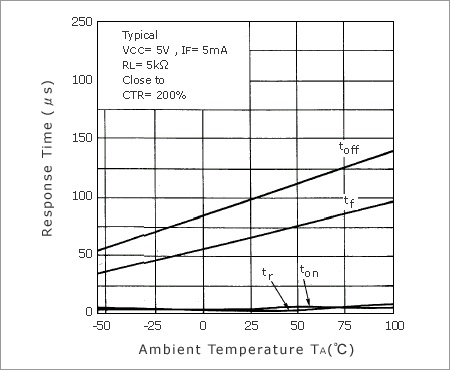
\includegraphics[width=0.8\linewidth]{ES_opto_CTR08.jpg}
            \caption{***}
            \label{es:fig_opto_CTR08}
          \end{figure}       
          Figure 8 shows an example of the variation in the response time according to the input
          current (IF).
          
          \begin{figure*}[ht!]
             \centering
             \subfloat[Response Time vs. IF Characteristics]{\label{ES:fig_opto_CTR08}
               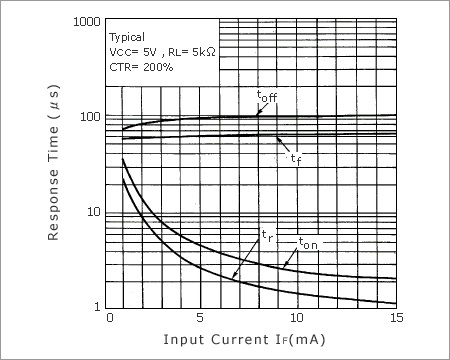
\includegraphics[width=0.4\textwidth]{ES_opto_CTR09.jpg}}
             \subfloat[Response Time vs. IF Characteristics]{\label{ES:fig_opto_CTR09}
               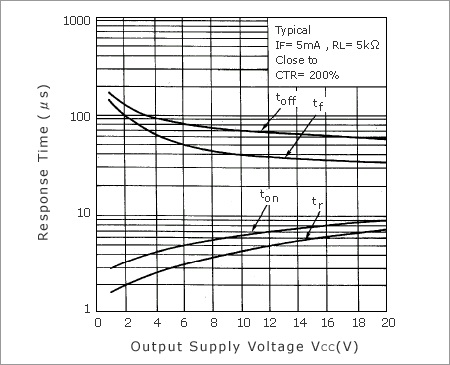
\includegraphics[width=0.4\textwidth]{ES_opto_CTR10.jpg}}   
             \caption{Závislost CTR na provozní době}
             \label{ES:fig_opto_tfvsIF}
          \end{figure*}          
       
          Figure 9 shows an example of the variation in the response time according to the power
          supply current (VCC).
          
      %-------------------Izolační parametry optronu------------------------------------------------
      \subsection{Izolační parametry optronu}
        V mnoha aplikacích je na izolační bariéry, kladen jen požadavek na kvalitní galvanického
        oddělení. Galvanické oddělení je obvykle efektivním prostředkem, jak potlačit šíření rušení
        mezi systémy, neboť jednoduše dokážeme přerušit zemní a jiné impedanční smyčky v obvodě.
        Kvalita tohoto oddělení je pak závislá na velikostech parazitních kapacit mezi vstupem a
        výstupem optoelektronického prvku. V těchto obvodech je optoelektronických vazebních prvků
        použito ačkoliv, oddělované signály mají stejný vztažný potenciál (např. GND). 
        
%         Izolace, na které jsou kladeny kromě funkčích také bezpečností požadavky, kritérium
%         jmenovitého izolačního napětí rozšířeno také další požadavky, které mohou vyplývat z norem
%         zabývajících se kooridancí izolací pro daný okruh aplikací, v jejichž souladu musí být dané
%         zařízení konstruované.  Účelem těchto norem je stanovit povrhové a vzdušné vzdálenosti pro
%         daný typ pracovní prostředí a druh konstručkního materiálu izolační bariéry.  a  tvořena
%         \emph{External creepage} je definována jako nejmenší vzdálenost vedenou přes izolační
%         bariéru po povrchu pouzda mezi vodivými prvky (vývody) optronu. \emph{external clearance}
%         je chápána jako nejmenší vzdušná vzdálenost vývodů.
        \begin{figure}[hb!]
          \centering
          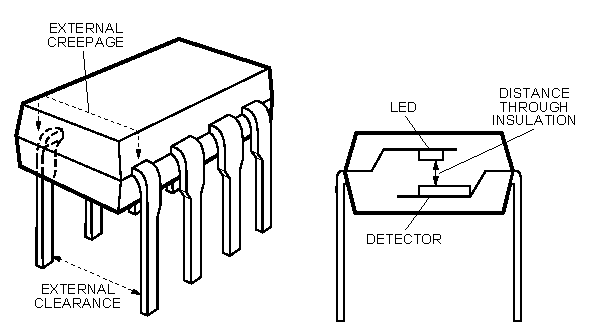
\includegraphics[width=0.7\linewidth]{optocoupler_clearance.pdf}
          \caption{K pojmu external creepage a clearance}
          \label{es:fig_optocoupler_clearance}
        \end{figure}

\ChapterBiblioList